\section{Implementation}\label{sec:umsetzung}
This chapter identifies technologies that can be used to implement the architecture presented in the last chapter.

\subsection{Mobile App}
The mobile app will be implemented for various mobile platforms such as Android, iOS, Windows Phone and as a web application. Furthermore, the mobile app can also be integrated into a loudspeaker.
\begin{itemize}
	\item \textsl{Speech Recording:} Recording a user's input does not require additional technology in most cases. Almost all mobile devices already have a microphone and the device \acs{sdk} provides an interface to access the microphone.
	\item \textsl{Speech Playback:} Also for playing a stream, the built-in speaker can be used via the devices \acs{sdk}.
	\item \textsl{Hotword Detection:} The following are technologies that can be used to detect a signal word on the mobile device:
	\begin{itemize}
		\item Snowboy Hotword Detection from Kitt.ai: Snowboy Hotword Detection is an Apache licensed software project for detecting a signal word. The signal word can be determined freely and the software project is optimized for embedded systems. According to the manufacturer Kitt.ai, the hotword detection under the smallest Raspberry Pi (single-core 700MHz ARMv6) is only consuming 10\% of the CPU \cite{SnowboyHotwordDetection}.
		\item Sensory's TrulyHandsfreeTM: Sensory's TrulyHandsfreeTM is a speech recognition optimized for recognizing single words or a signal word. It also shows very good results in environments with lots of background noise. The vocabulary to be recognized can be created by Sensory's Grammar Tool. Sensory's TrulyHandsfreeTM is available for Android, iOS, QNX, Windows and microcontrollers \cite{TrulyHandsfreeTM}.
		\item Pocketsphinx from \acs{cmu} Sphinx: Sphinx is a \ac{cmu} research project dealing with speech recognition. Sphinx is based on the Open Source license and can therefore be used freely as long as it is acknowledged that it is a software of \ac{cmu}. Pocketsphinx, as well as Sensory's TrulyHandsfreeTM, has been optimized to recognize single words or a signal word \cite{Pocketsphinx}.
	\end{itemize}
\end{itemize}

\subsection{Repository}
The repository can be implemented by a web server. This web server provides on the one hand different runtime environments and on the other hand apps for the language assistant for download. The runtime environments can be offered in the following formats:
\begin{itemize}
	\item \textsl{VMWare Image:} The VMWare image already contains a preinstalled operating system as well as all necessary packages for the language assistant. A user must import this image into their VMWare environment (VMWare vSphere, Workstation, Player) and make only small network configurations. This environment is easy to use and requires the least amount of configuration. In addition, the user has the option of transferring the virtual machine to another server or taking snapshots. Snapshots are images of a virtual machine that reflect a particular state. This can easily jump back to the last functional snapshot in case of a misconfiguration \cite{VMWare}.
	\item \textsl{Docker Image:} The Docker Image is a configuration file for a container environment. This configuration file contains all packages and configurations for the language assistant to be installed. If this configuration file is started in a container environment, the packages are automatically installed and the language assistant is configured. The user only has to make network settings to use the language assistant \cite{Docker}.
	\item \textsl{\acs{iso}-Image:} The \acs{iso}-Image provides the user with the most flexibility and configuration. The user can decide whether to install the runtime environment physically or virtualized. Furthermore, this is not tied to virtualization software like VMWare. It can be virtualized on a private or public cloud. A public cloud relieves the user of tasks such as visualization, backups, reliability and load balancing. Possible providers are \ac{aws} with Amazon EC2 \cite{AWSAmazonEC2}, Microsoft Azure \ cite {MicrosoftAzure}, and IBM Bluemix \cite{IBMBluemix}. The \acs{iso}-Image also contains all the necessary packages for the language assistant. The user is guided through a wizard during the installation of the \acs{iso}-Image, where all configurations are made.
\end{itemize}

\subsection{Runtime Environment}
\subsubsection{Speech Processing}
In the runtime environment, speech processing processes are performed. There are two ways to perform these processes, either locally on the runtime environment or through the use of voice-based cloud services. The advantages and disadvantages as well as possible technologies of these possibilities are explained below.
\begin{itemize}
	\item \textsl{Cloud-based Speech Processing:} The use of voice-based cloud services for speech processing provides the best possible performance. The language processing is based on a \ac{ai}, which improves with input data. Because cloud services are used by many applications, \ac{ai} provides a large amount of input data. The disadvantage of this is that a user's \ac{ai} input data describing its context is used to improve the \ac{ai}. Thus, the privacy is not optimally protected. Furthermore, the use of cloud services incurs costs. The following providers offer voice-based cloud services:
	\begin{itemize}
		\item \ac{aws}: Amazon offers many voice-based cloud services. Amazon Comprehend is a service for \ac{nlu}, gaining insight into the context and relationships of a text \cite{AmazonComprehed}. With Amazon Translate, texts, web pages, and applications can be translated naturally and accurately \cite{AmazonTranslate}. Amazon Transcript can convert speech to text and Amazon Polly text to speech \cite{AmazonTranscript} \cite {AmazonPolly}. Amazon Lex can create conversation interfaces for applications. A chat bot serves as a  interface and can generate the corresponding answer to a specific input. Amazon Lex uses the same deep learning algorithms as voice assistant Alexa from Amazon \cite{AmazonLex}.
		\item Microsoft Azure: Microsoft Azure offers cognitive services, including text to speech, speech to text, text translation, and \ac{nlu} services. It also offers a speaker recognition and spelling correction service \cite{MicrosoftAzureCognitiveServices}. Speech recognition is an important part of the concept of the voice assistant presented in this article. Through this service, a user can be authenticated.
		\item IBM Watson: IBM Watson also offers voice-based cloud services for speech to text and text to speech conversion. Furthermore, a service for \ac{nlu} and \ac{nlc} is offered. By \ac{nlc} the intention of an input can be determined. With Watson Assistant a Chat bot can be realized \cite{IBMWatsonSpeechServices}.
	\end{itemize}
	\item \textsl{Local Speech Processing:} The use of local speech processing in the runtime environment provides better control of the user's privacy. This requires significantly more resources on the runtime environment, and performance is usually worse than using voice-based cloud services. There are some vendors that offer frameworks for local language processing. Including open-source projects, resulting in no costs for the use.
	\begin{itemize}
		\item Nuance:Nuance has been working on speech processing solutions for over 25 years, focusing on integrating these solutions into mobile devices such as smartphones or cars. Among other things, solutions for speech to text and text to speech conversions and to create a chat bot are offered \cite{Nuance}. 
		\item Mozilla: Mozilla is launching the Common Voice project, an initiative to help teach machines the way real people speak. This initiative is still under development. Currently, records are being collected to improve the \ac{ai}. The initiative is considered as an open source project and each person can add records for improvement of the \ac{ai}. For this purpose, Mozilla has created a website and mobile app with the contributor to review records or input data \cite{MozillaCommonVoice}. The potential of this initiative will only become apparent after the end of development.
		\item Kaldi: Kaldi is a speech recognition toolkit that is freely available under the Apache license. Kaldi aims to deliver software that is flexible and extensible \cite{Kaldi}. The project is managed on GitHub, so developers can help improve the toolkit.
		\item CMUSphinx: CMUSphinx offers with Pocketsphinx a speaker-independent continuous speech recognition. Pocketsphinx is an open source project and is managed on GitHub. Pocketsphinx can be used in mobile devices, offering a version for smartwatches that does not require an internet connection. Finished models for the \ac{ai} are offered, but even own models can be trained \cite{Pocketsphinx}.
	\end{itemize}
\end{itemize}

\subsubsection{Configuration Environment}
The configuration environment can be realized by a web application. The user can configure his voice assistant via any device with a browser. Furthermore, these configurations can also be done with the mobile app. Figure \ref{fig: prototype} shows a prototype of what this mobile app might look like. In doing so, a user can view his context and determine which contextual information of apps may be used. The user can manipulate his context if certain information is needed by an app; he does not want to divulge these for reasons of privacy. Thus, the user has full control over his data.

\begin{figure}[!ht]
	\centering
	\begin{subfigure}{0.32\linewidth}
		\centering
		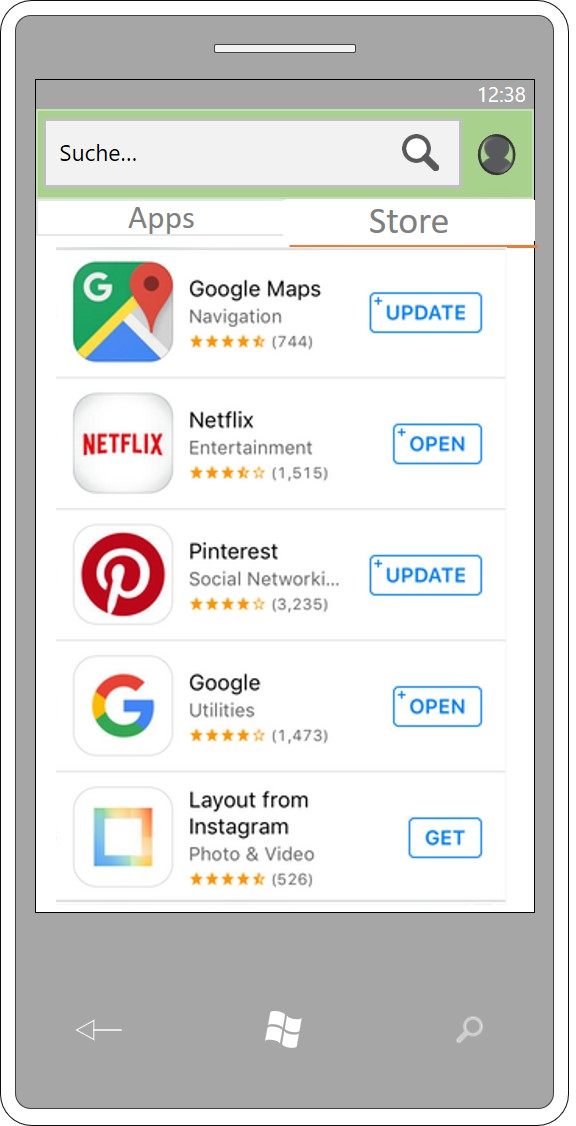
\includegraphics[width=1\linewidth]{Picture/App-Store}
		\caption{Mobile App - Store}
		\label{fig:prototyp1}
	\end{subfigure}%
	\begin{subfigure}{0.32\linewidth}
		\centering
		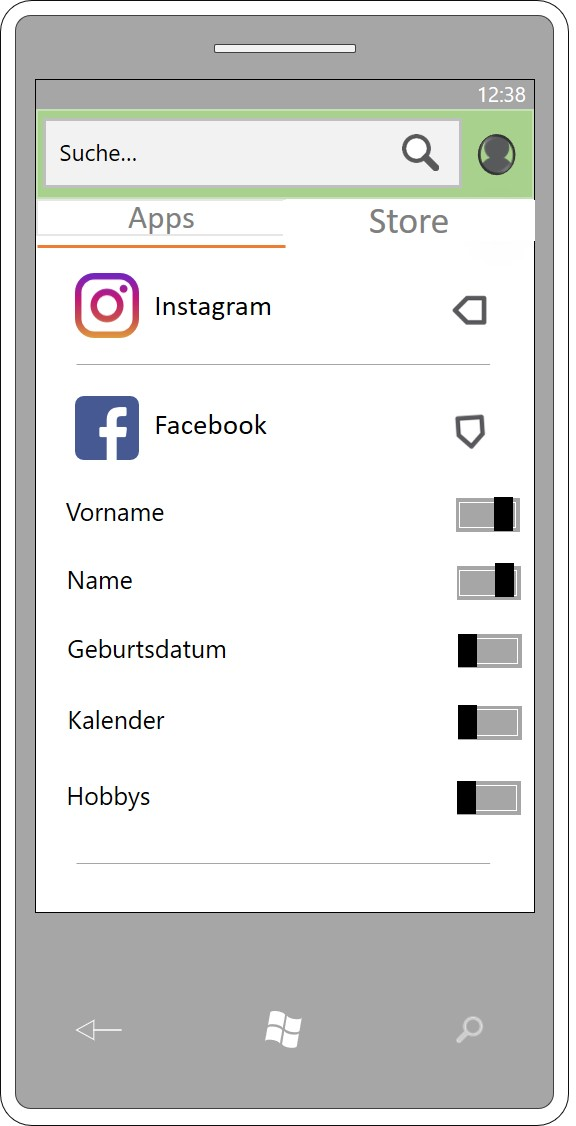
\includegraphics[width=1\linewidth]{Picture/App-Settings}
		\caption{Mobile App - Settings}
		\label{fig:prototyp2}
	\end{subfigure}
	\begin{subfigure}{0.32\linewidth}
		\centering
		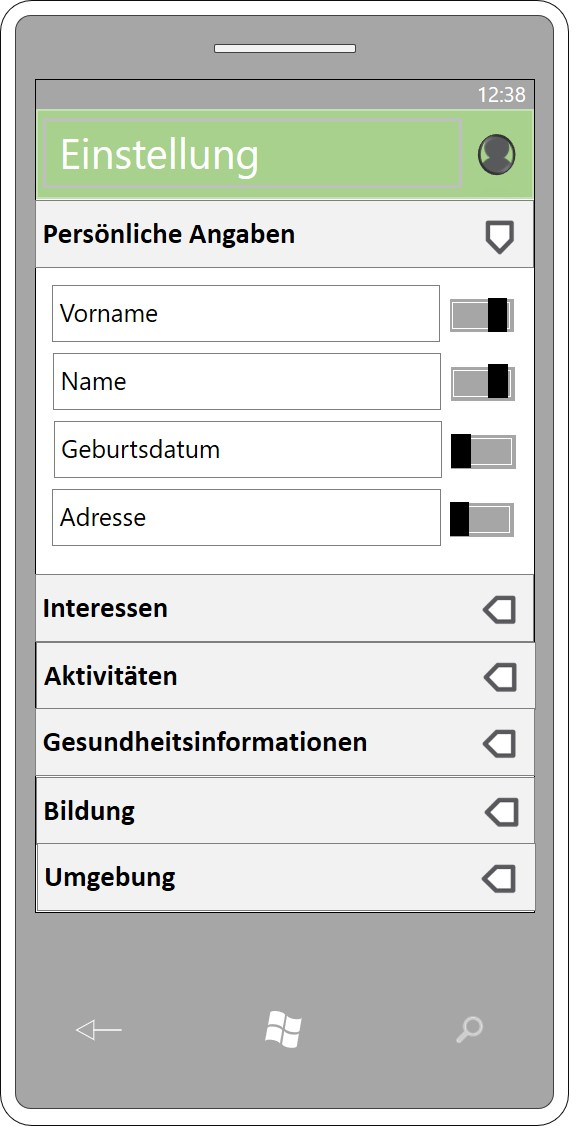
\includegraphics[width=1\linewidth]{Picture/App-Kontext}
		\caption{Mobile App - User Context}
		\label{fig:prototyp3}
	\end{subfigure}%
	\caption{Prototyp of the mobile App}
	\label{fig:prototyp}
\end{figure}











